\documentclass[10pt,twocolumn,letterpaper]{article}

\usepackage{cvpr}
\usepackage{times}
\usepackage{epsfig}
\usepackage{graphicx}
\usepackage{amsmath}
\usepackage{amssymb}
\usepackage{graphicx}
\usepackage{subfig}
\usepackage{url}

\usepackage[breaklinks=true,bookmarks=false]{hyperref}

\cvprfinalcopy
\begin{document}

%%%%%%%%% TITLE
\title{Friendly Streets: A Street View Classifier for Cautious Cyclists}

\author{Josh Sennett\\
University of Massachusetts, Amherst\\
{\tt\small jsennett@umass.edu}
\and
Evan Rourke\\
University of Massachusetts, Amherst\\
{\tt\small erourke@umass.edu}
}

\maketitle

%%%%%%%%% ABSTRACT
\begin{abstract}
The goal of this project is to classify street-view images as ``bike-designated'' or ``not''. Existing research has shown that convolutional neural networks (CNNs) are well-suited for scene classification and object detection, but have not been applied to classify bike-designation. The three contributions of this work are 1) to create a tool to generate high-quality datasets of street-view images labeled as bike-designated or not; 2) to develop a neural network to predict this label; and, 3) to establish a human baseline with which to compare the accuracy of our neural network. By fine-tuning a pre-trained ResNet neural network, we achieve 68.0\% overall accuracy on a test set of 3,454 unseen images, outperforming a human benchmark of 59.7\% on 1,296 images.
\end{abstract}

%%%%%%%%% INTRODUCTION
\section{Introduction}
\label{sec:intro}

Cyclists depend on routing applications to find safe and enjoyable bike routes. In these applications, roads may be ``bike-designated'' based on data from public records, privately-owned data sources, or open-source communities. The classification of bike-designation is often outdated, inaccurate, or unavailable, presenting a challenge for mapping software and cyclists to plan safe and optimal routes.

To approach this problem, we develop a convolutional neural network to classify street-view images of roads as bike-designated or not. We train our network on a dataset of street-view images labeled ``bike-designated'' or ``not'', which we generated by integrating OpenStreetMap \cite{osm} road classifications with Google's Street View API \cite{googlesv}.

``Bike-designation'' refers to whether a road contains infrastructure to make a road safer or more enjoyable for cyclists. OpenStreetMap, which we use as our source of road classification data, defines bike-designation as whether a roadway (for motor-vehicles) contains either a bike lane (a lane within a roadway) or a bike path (a lane alongside a roadway, but separated by a barrier). Bike-designated roads may also have shared-road arrows (``sharrows''), colored bike lanes, physical barriers, and cautionary (``share the road'') street signs.

\begin{figure}[t]
\begin{center}
	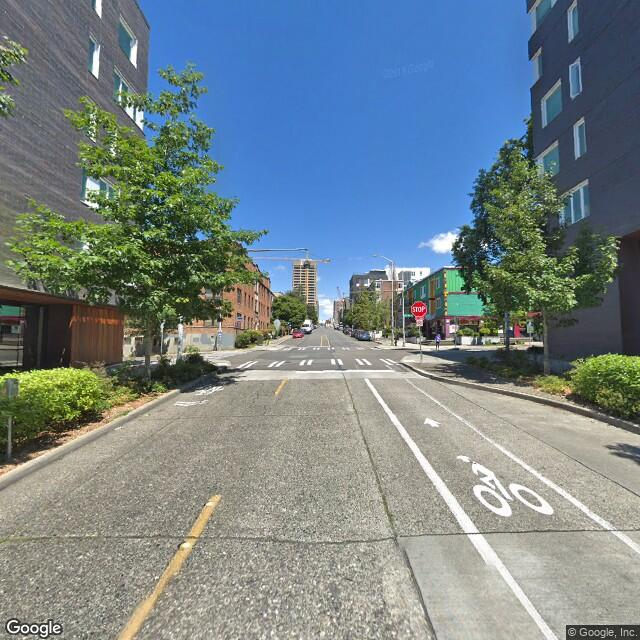
\includegraphics[width=0.4\linewidth]{intro1.jpg}
	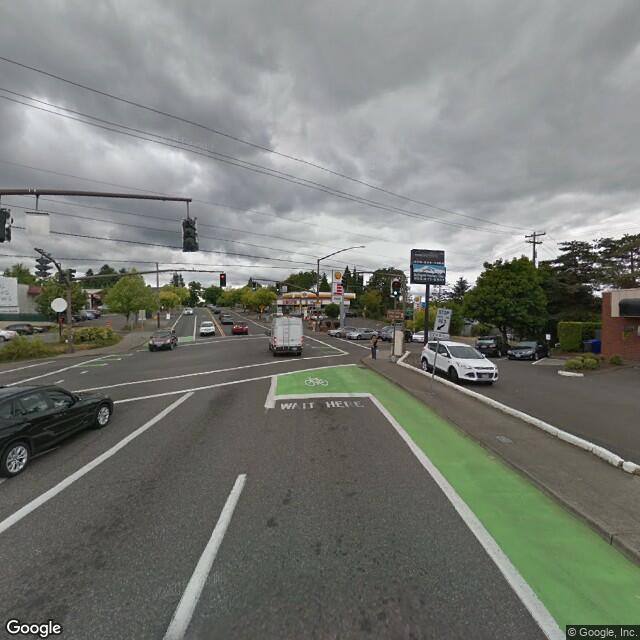
\includegraphics[width=0.4\linewidth]{intro7.jpg}
	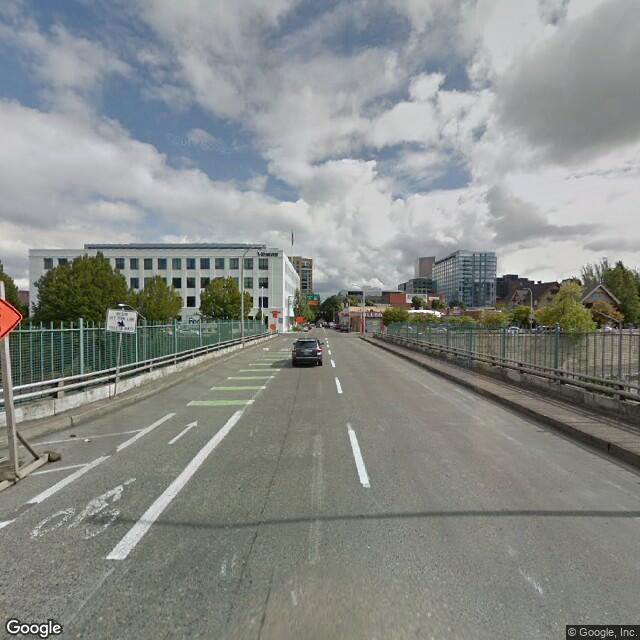
\includegraphics[width=0.4\linewidth]{intro4.jpg}
	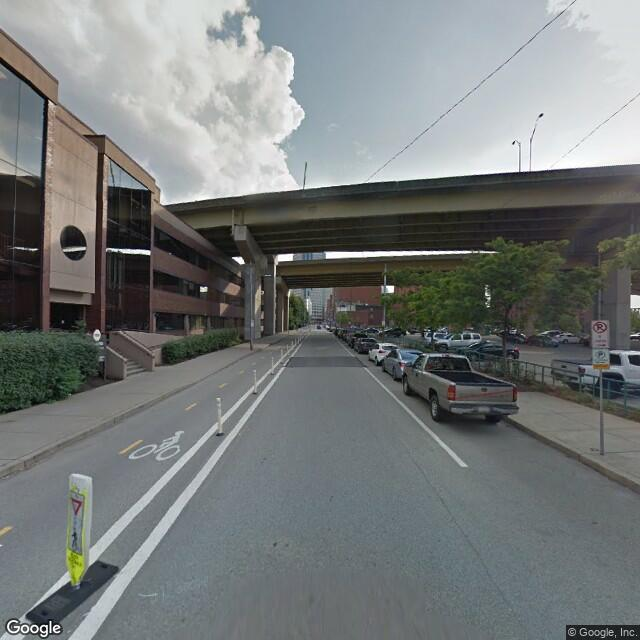
\includegraphics[width=0.4\linewidth]{intro5.jpg}
\end{center}
   \caption{Shared road markings (``sharrows''), colored bike lanes, and barriers are common features of bike-designated roads.}
\label{fig:long}
\label{fig:onecol}
\end{figure}


\begin{figure*}
  \centering
  \subfloat[Bike-designated]{
  	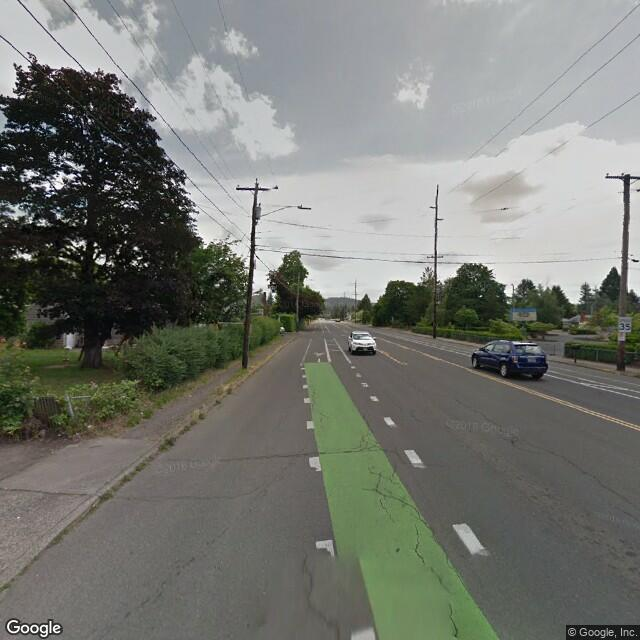
\includegraphics[width=0.1\textwidth]{intro2.jpg}\label{fig:f1}
  	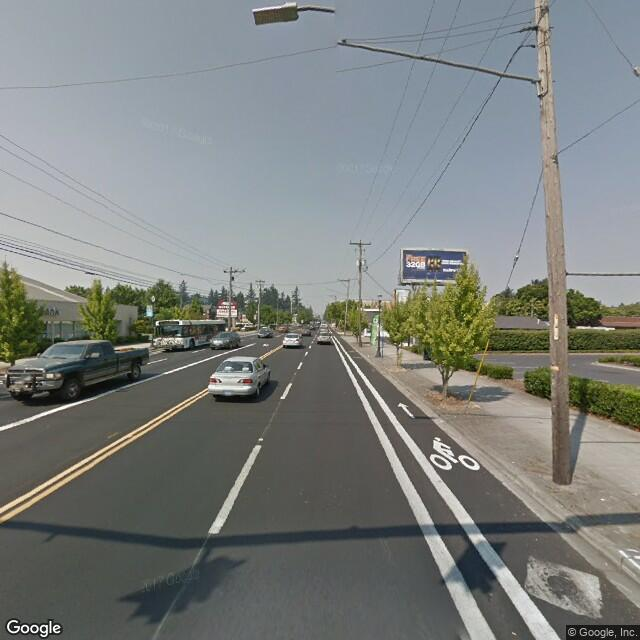
\includegraphics[width=0.1\textwidth]{intro3.jpg}\label{fig:f1}
  	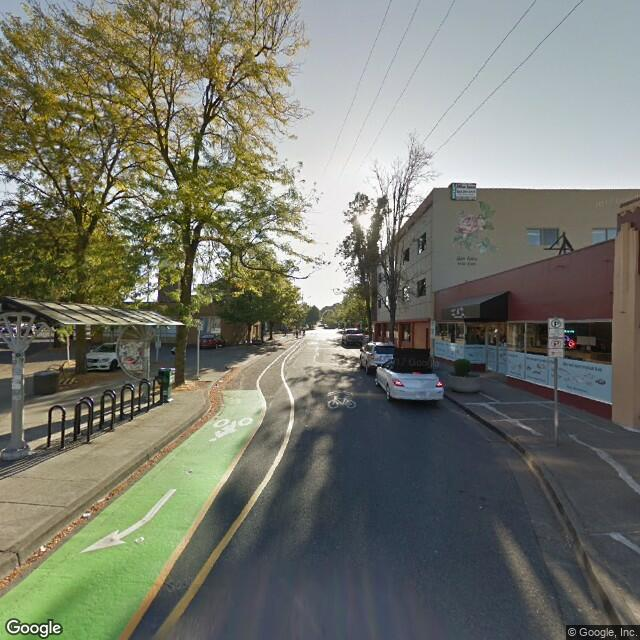
\includegraphics[width=0.1\textwidth]{intro6.jpg}\label{fig:f1}
  	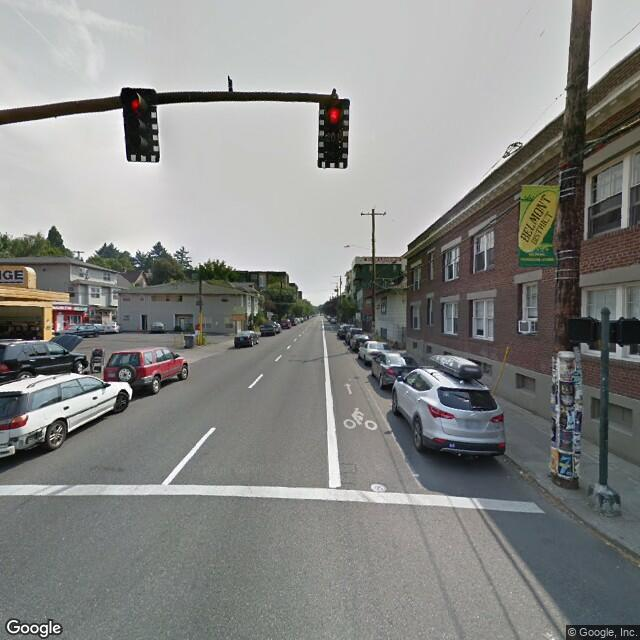
\includegraphics[width=0.1\textwidth]{intro8.jpg}\label{fig:f1}
	}
  \hfill
  \subfloat[Not bike-designated]{
  	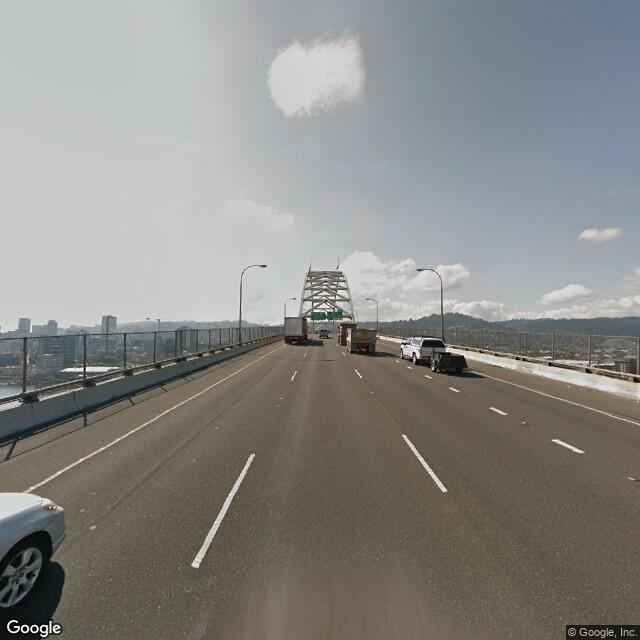
\includegraphics[width=0.1\textwidth]{intro9.jpeg}\label{fig:f1}
  	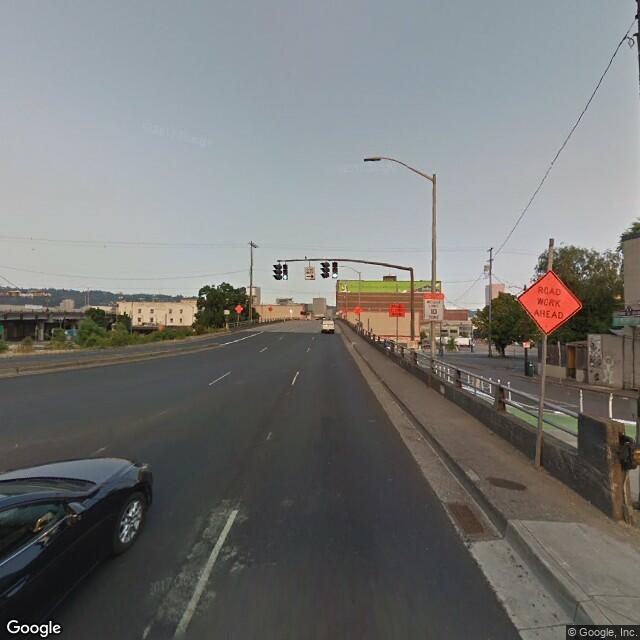
\includegraphics[width=0.1\textwidth]{intro10.jpg}\label{fig:f1}s
  	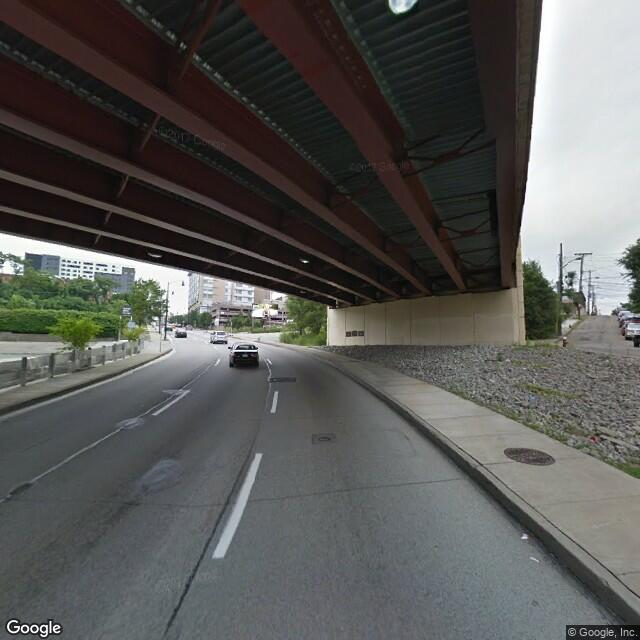
\includegraphics[width=0.1\textwidth]{intro11.jpg}\label{fig:f1}
  	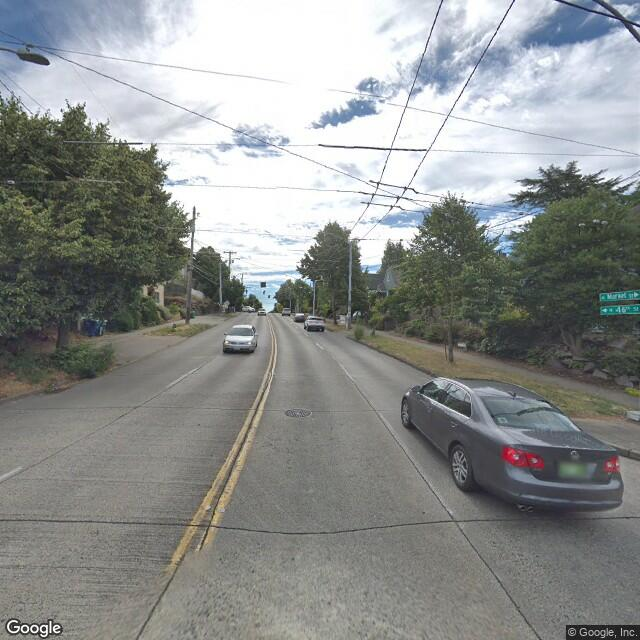
\includegraphics[width=0.1\textwidth]{intro12.jpeg}\label{fig:f1}
  }
  \caption{Example street-view images of bike-designated and not bike-designated roads.}
\end{figure*}

Developing a bike-designation street-view image classifier faces several challenges. First, there is no existing public, large-scale database of street-view images with the bike-designation label. Second, bike-designated roads contain a variety of different types of cycling infrastructure, and each type of infrastructure may look different depending on which city and country the road pertains to. Third, street-view images may not be positioned or oriented correctly to capture the relevant features. Last, street-view images are taken in real-world settings, and face several factors that decrease image quality including feature occlusion, background clutter, differences in illumination, and blur.

To overcome the first challenge, we generate a labeled dataset of street-view images by integrating OpenStreetMap road classification data with Google's Street View API. To overcome the remaining challenges, we develop a convolutional neural network to classify street-view images as bike-designated or not. Previous research has demonstrated the effectiveness of CNNs for scene understanding and object detection in real-world settings, where viewpoint variation, occlusion, background clutter, illumination, and intra-class variation are expected [cite 231]. 

The paper is structured as follows. Section \ref{sec:background} presents related research. Section \ref{sec:approach} explains our approach to developing a labeled dataset, neural network, and human baseline. Section \ref{sec:experiments} contains the results of our experiments to improve our network's performance. Section \ref{sec:conclusion} concludes with lessons learned and directions for future research.

%%%%%%%%% RELATED WORK
\section{Background and Related Work}
\label{sec:background}

\subsection{Scene Classification}
Convolutional neural networks have been widely successful in object classification tasks \cite{krizhevsky2012imagenet}. Trained on massive datasets, these networks have been able to nearly achieve or even exceed human performance benchmarks.

Scene classification, however, is a more challenging, generalized task than object classification: a scene class may be correlated with the presence of objects, but such objects may appear in other scene classes. Correctly classifying a scene depends not only on objects but also attributes (relating to spatial envelope, materials, lighting, and textures).

Xiao et al. developed the SUN Database, the first large-scale scene understanding database with 899 scene categories and over 130,000 labeled images\cite{xiao2010sun}. Shortly thereafter, Patternson and Hays developed the first large-scale scene attributes dataset and demonstrate the predictive power of attributes for classifying scenes \cite{6247998}. Most recently, Zhou et al. develop the Places database, a database of 434 scene categories and over 10 million scene images \cite{DBLP:journals/corr/ZhouKLTO16}. Using the Places database, Zhou et al. surpassed previous scene classification benchmarks using VGG, GoogLeNet, AlexNet, and ResNet convolutional neural networks. 

\subsection{Street View Images}
Several researchers have used Google Street View images as a source of natural images; Google Street View cars take panoramic photos along roads, providing a rich source of images of outdoor scenes. Netzer et al use Street View images to generate the Street View House Number dataset for digit classification. Similarly, Slavkovikj et al. use Street View images to develop a road-texture dataset for classification [cite]. Gebru et al. develop a car brand classifier [cite], and Hershey and Wulfe use deep learning to recognize geo-location from city Street View images.

%%%%%%%%% APPROACH
\section{Approach}
\label{sec:approach}


\subsection{Data}
To generate a labeled dataset of bike-designated street-view images, we created a tool to integrate OpenStreetMap road classifications with Google's Street View API. This tool does the following:
\begin{enumerate}
\item Download OpenStreetMap data for a particular region
\item Extract road segments (way elements) for this region using particular criteria
\item Extract road points (node elements) for these ways using particular criteria
\item Calculate road orientation for each for these nodes
\item Query Google's Street View API using node coordinates and road orientation
\item Save the street-view image with the road classifications
\end{enumerate}
Specifically, to create a dataset of bike-designated images, we did the following.

In step 1, we used OpenStreetMap data for four cities: Boulder, Pittsburgh, Portland, and Seattle. We chose these regions because of the quality and availability of bike-designation for roads in these cities, and because these cities have near-balance between bike-designated and non-designated roads (in total, 57\% and 43\%).

In step 2, we filtered road segments to only include road types ``motorway'', ``primary highway'', ``secondary highway'', and ``tertiary highway''. Other segment types included non-road segments not relevant to our analysis such as footpaths and bike-paths, as well as residential roads, which were often unlabeled with road classifications.

In step 3, we filtered nodes to only include the midpoint of each road. Given the cost of the Google Street View API (\$7 per 1000 images), we could not capture Street View images at all millions of nodes of all relevant highways. Nodes are typically several meters apart; so, capturing Street View images at adjacent nodes will result in similar images with a slightly shifted camera perspective. Extracting a single image for each road segment (rather than extracting multiple images at a subset of road segments) increases image heterogeneity while keeping our API costs reasonable.

In step 4, we determine the required camera orientation such that each image is pointed in the direction of the road. To do so, we calculate the geodesic azimuth (angular distance from north) between a node and the subsequent node. For one-way roads, we orient the camera to face in the forward-direction of the road.

In step 5, we query the API to determine if a Street View image is available for the given coordinate in a radius of 10 meters. We found that reducing the search radius to 10 meters decreased the chance that images of nearby (but different) roads were not accidentally downloaded in the case that a road did not have street-view images. Then, if an image is available, we download a 640x640 image using the node coordinate and the calculated camera orientation.

\subsection{Neural Network}
why we chose pre-trained places365, why we chose to fine-tune, how we came up with the final model
pictures of training/val loss accuracy

\subsection{Human Benchmark}
NOTE: INCLUDE A SCREENSHOT OF THE HUMAN BENCHMARK INTERFACE
if you have per-person scores, maybe include the standard deviation of scores and average images classified per person


%%%%%%%%% EXPERIMENTS
\section{Experiments}
\label{sec:experiments}
different models: fc1, fc2, fc3, w/wout dropout, leakyrelu
different optimizers: adam, SGD with momentum + L2 reg
hyperparameter search: learning rate, reg strength, hidden layer size
how we chose: trained on 10\% of dataset, looked at loss/acc curves

show images, CAM, attributes, with our prediction
top accuracy for our models (68\%)

final model: fc3 (400 units?), 10\% dropout and leakyrelu, SGD + momentum, L2 reg

This section begins with what kind of experiments you're doing, what kind of dataset(s) you're using, and what is the way you measure or evaluate your results. It then shows in details the results of your experiments. By details, we mean both quantitative evaluations (show numbers, figures, tables, etc) as well as qualitative results (show images, example results, etc).

\begin{figure}[t]
\begin{center}
	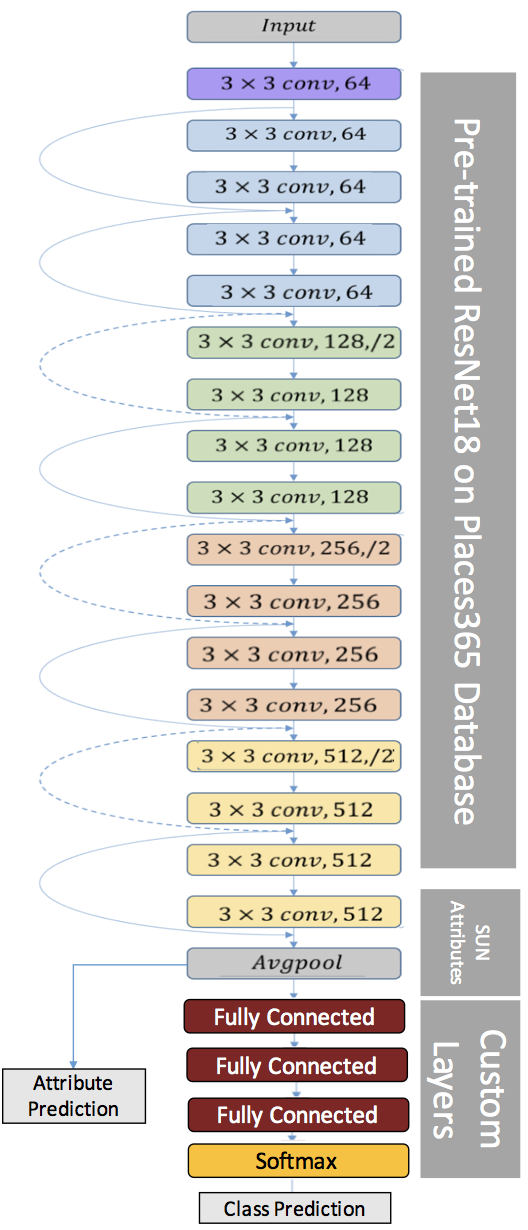
\includegraphics[width=.7\linewidth]{model.png}
\end{center}
   \caption{Final model: Pre-trained ResNet18 with three fine-tuned fully-connected layers.}
\label{fig:long}
\label{fig:onecol}
\end{figure}



%%%%%%%%% CONCLUSION
\section{Conclusion}
\label{sec:conclusion}
What have you learned? 

Suggest future ideas.\\

List and number all bibliographical references at the end of your paper. When referenced in the text,
enclose the citation number in square brackets, for
example. \\

TODO: add the rest of the citations here from cs682\_final\_report.bib

\cite{slavkovikj2014image}
\cite{patterson2014sun}
\cite{rundle2011using}
\cite{zhou2017places}
\cite{DBLP:journals/corr/ZhouKLOT14}
\cite{DBLP:journals/corr/Wang15l}
\cite{DBLP:journals/corr/HeZRS15}
\cite{DBLP:journals/corr/ZagoruykoK16}
\cite{DBLP:journals/corr/ZhouKLTO16}
\cite{koehrsen2018blog}

{\small
\bibliographystyle{ieee}
\bibliography{cs682_final_report.bib}
}

\end{document}
